% Created 2022-03-02 水 23:46
% Intended LaTeX compiler: pdflatex
\documentclass[lualatex,a4paper,12pt,report,ja=standard]{bxjsarticle}
\usepackage{bm}
\usepackage[sumlimits]{amsmath}
\usepackage{xcolor}
\usepackage{makeidx}
%\usepackage{newtxtext,newtxmath}
\usepackage{graphicx}
\usepackage[hidelinks,colorlinks=true,linkcolor=black]{hyperref}

%\usepackage[top=30truemm,bottom=30truemm,left=37truemm,right=18truemm]{geometry}
%%%%%% generate by 'org-latex-classes "luareport" %%%%%%


\usepackage{minted}
\setcounter{secnumdepth}{4}
\author{Osada Yuma}
\date{\today}
\title{Correspondence between R+ggplot2 and gnuplot.}
\hypersetup{
 pdfauthor={Osada Yuma},
 pdftitle={Correspondence between R+ggplot2 and gnuplot.},
 pdfkeywords={},
 pdfsubject={},
 pdfcreator={Emacs 28.0.50 (Org mode 9.5)}, 
 pdflang={English}}
\begin{document}

\maketitle
\tableofcontents

\section{はじめに}
\label{sec:org789026b}
\subsection{文書}
\label{sec:orgd114d23}
ファイル
\url{https://github.com/osada-yum/examples} のR\textsubscript{ggplot2}
Emacsのorg-babelに対応している.
\subsection{実行環境}
\label{sec:org848ad7a}
\begin{itemize}
\item Ubuntu 20.04
\item org-9.5.2 on Emacs-28.0.50
\end{itemize}
\section{やりたいこと}
\label{sec:orgd7c7dc3}
\begin{itemize}
\item gnuplot並に簡単にプロットをしたい.
\end{itemize}
\section{gnuplotから引っ越す}
\label{sec:org1ba8283}
\begin{itemize}
\item gnuplotは簡易的にデータを可視化するには取り回し易い.
\texttt{gnuplot filename} でOK.
\item データの加工は面倒.
できなくはない.
\end{itemize}
\subsection{R+ggplot2の利点}
\label{sec:org42bc43c}
\begin{itemize}
\item Rの機能が使える.
\begin{itemize}
\item ファイルからデータを読み込んで加工してプロットするのが楽.
\item \texttt{head(data)} とかでデータの上をちょっと覗いたり,
\texttt{summary} で統計を取ったりしやすい.
\end{itemize}
\item プロットの設定を弄りやすい.

テーマを変えたりプロットの枠を変えたりとか.
\item 別のRパッケージでより便利になる.

\texttt{patchwork} (プロットを並べられる)とか

\texttt{gganimate} (.gif作れる)とか
\item ggplot2単体ではプロットをマウスで動かせない.

\texttt{ggplotgui} (ブラウザ上でプロットを動かせる)とかを使えば可能.
\item マルチバイト文字が使える.

gnuplot では使えない?
\end{itemize}
\subsection{R+ggplot2の欠点}
\label{sec:orge9f3436}
\begin{itemize}
\item 日本語の文書が少ない.

とりあえず, `` \texttt{R ggplot2} '' とかで検索?
\item \texttt{gnuplot} に比べると行数が増える.
\end{itemize}
\section{デモ}
\label{sec:org8f6ea8e}
一部の画質が粗いのは, おそらくorg-babelで出力しているから.
\mintinline[frame=lines,framesep=2mm,linenos=true,baselinestretch=1.2,fontsize=\footnotesize,breaklines]{r}{ggsave()} 関数を使えば dpi を弄れるので問題なし.
\subsection{ファイルをプロットしたい}
\label{sec:org78eb7ab}
\subsubsection{emacsのorg-babel用の設定}
\label{sec:org377f943}
\begin{minted}[frame=lines,framesep=2mm,linenos=true,baselinestretch=1.2,fontsize=\footnotesize,breaklines]{common-lisp}
(org-babel-do-load-languages
 'org-babel-load-languages
 '((emacs-lisp . t)
   (gnuplot    . t)
   (R          . t)))
\end{minted}

\subsubsection{ファイルの中身}
\label{sec:org410f17c}
\texttt{sin.dat}
\begin{minted}[frame=lines,framesep=2mm,linenos=true,baselinestretch=1.2,fontsize=\footnotesize,breaklines]{bash}
cat sin.dat
\end{minted}

\begin{center}
\begin{tabular}{rr}
1 & 0.3271947\\
2 & 0.6183698\\
3 & 0.84147096\\
4 & 0.971937\\
5 & 0.99540794\\
6 & 0.9092974\\
7 & 0.7230859\\
8 & 0.45727262\\
9 & 0.14112\\
10 & -0.19056797\\
\end{tabular}
\end{center}

\texttt{cos.dat}
\begin{minted}[frame=lines,framesep=2mm,linenos=true,baselinestretch=1.2,fontsize=\footnotesize,breaklines]{bash}
cat cos.dat
\end{minted}

\begin{center}
\begin{tabular}{rr}
1 & 0.9950042\\
2 & 0.9800666\\
3 & 0.9553365\\
4 & 0.921061\\
5 & 0.87758255\\
6 & 0.8253356\\
7 & 0.7648422\\
8 & 0.6967067\\
9 & 0.62161\\
\end{tabular}
\end{center}

\subsubsection{gnuplotなら}
\label{sec:org2457cfb}
\begin{itemize}
\item 凄い簡単.
\item データを可視化したいだけなら, これだけでOK.
\end{itemize}
\begin{minted}[frame=lines,framesep=2mm,linenos=true,baselinestretch=1.2,fontsize=\footnotesize,breaklines]{gnuplot}
plot "sin.dat"
\end{minted}

\begin{center}
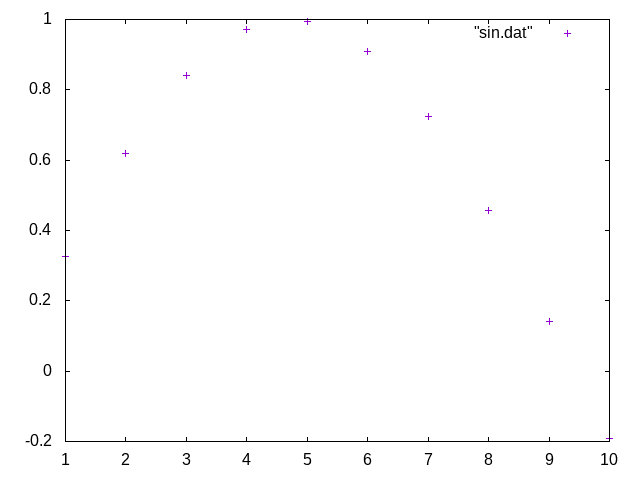
\includegraphics[width=0.8\textwidth]{figure/sin_gnuplot.png}
\end{center}

\subsubsection{R+ggplot2で愚直にプロット}
\label{sec:org995a150}
\begin{itemize}
\item \texttt{ggplot2} をインストールする.
\end{itemize}
\begin{minted}[frame=lines,framesep=2mm,linenos=true,baselinestretch=1.2,fontsize=\footnotesize,breaklines]{r}
install.packages("ggplot2")
\end{minted}

\begin{itemize}
\item \texttt{ggplot2} のライブラリを読み込む.
\end{itemize}
\begin{minted}[frame=lines,framesep=2mm,linenos=true,baselinestretch=1.2,fontsize=\footnotesize,breaklines]{r}
library(ggplot2)
\end{minted}

\begin{itemize}
\item \texttt{read.table} 関数でファイルを読み込む.
\item `` \texttt{.} '' は名前の一部であり, メソッドアクセス演算子ではない.
\item 列の名前はV1, V2, \ldots{}となっている.
\texttt{colnames} 関数で変更することも可能.
\end{itemize}
\begin{minted}[frame=lines,framesep=2mm,linenos=true,baselinestretch=1.2,fontsize=\footnotesize,breaklines]{r}
d_sin <- read.table("sin.dat", header = F)
head(d_sin, n = 2)
\end{minted}

\begin{center}
\begin{tabular}{rr}
V1 & V2\\
\hline
1 & 0.3271947\\
2 & 0.6183698\\
\hline
\end{tabular}
\end{center}

\begin{itemize}
\item \texttt{ggplot()} と部品(\texttt{geom\_point} とか)を \texttt{+} で組み合わせてプロットする.
\item 以下も可能.
\begin{itemize}
\item \mintinline[frame=lines,framesep=2mm,linenos=true,baselinestretch=1.2,fontsize=\footnotesize,breaklines]{r}{ggplot(data = d_sin) + geom_point(aes(x = V1, y = V2))}

\mintinline[frame=lines,framesep=2mm,linenos=true,baselinestretch=1.2,fontsize=\footnotesize,breaklines]{r}{geom_point(aes(x = V1, y = V3))}を追加すれば別の列もプロットできる.
\item \mintinline[frame=lines,framesep=2mm,linenos=true,baselinestretch=1.2,fontsize=\footnotesize,breaklines]{r}{ggplot(data = d_sin, aes(x = V1, y = V2)) + geom_point()}

\mintinline[frame=lines,framesep=2mm,linenos=true,baselinestretch=1.2,fontsize=\footnotesize,breaklines]{r}{geom_line()}で点と線を一緒にプロットできる.
\item \mintinline[frame=lines,framesep=2mm,linenos=true,baselinestretch=1.2,fontsize=\footnotesize,breaklines]{r}{ggplot() + geom_point(data = d_sin, aes(x = V1, y = V2))}

\mintinline[frame=lines,framesep=2mm,linenos=true,baselinestretch=1.2,fontsize=\footnotesize,breaklines]{r}{geom_point(data = another, aes(x = V5, y = V1))}で別の \texttt{data.frame} のデータも一緒にプロットできる
\end{itemize}
\end{itemize}
\begin{minted}[frame=lines,framesep=2mm,linenos=true,baselinestretch=1.2,fontsize=\footnotesize,breaklines]{r}
plt <- ggplot(data = d_sin) + geom_point(aes(x = V1, y = V2))
plt
\end{minted}

\begin{center}
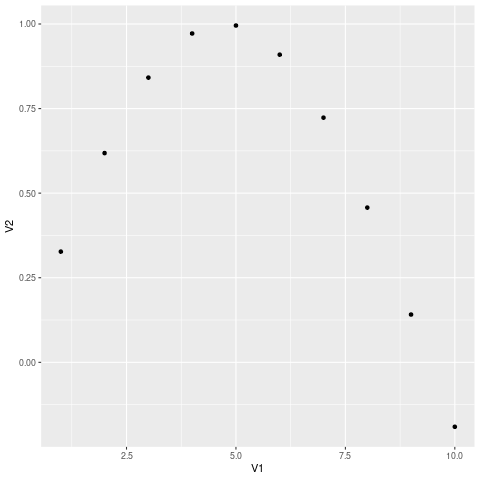
\includegraphics[width=0.8\textwidth]{figure/sin_ggplot2.png}
\end{center}

\subsubsection{gnuplotに似せる}
\label{sec:orgc968bdf}
\begin{enumerate}
\item themeの設定
\label{sec:org2808145}
\begin{minted}[frame=lines,framesep=2mm,linenos=true,baselinestretch=1.2,fontsize=\footnotesize,breaklines]{r}
plt_theme <- plt + theme_bw()
plt_theme
\end{minted}

\begin{center}
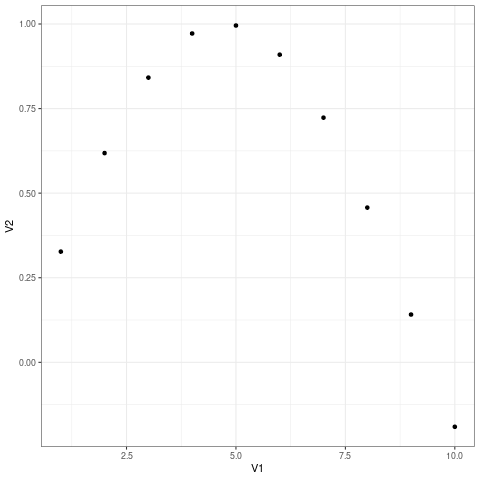
\includegraphics[width=0.8\textwidth]{figure/sin_ggplot2_theme.png}
\end{center}

\item breakの設定
\label{sec:org7fc7844}

(\texttt{gnuplot} でいうticks.)
\begin{minted}[frame=lines,framesep=2mm,linenos=true,baselinestretch=1.2,fontsize=\footnotesize,breaklines]{r}
plt_breaks <- plt_theme +
  scale_x_continuous(breaks = seq(from = 1.0, to = 10.0, by = 1.0)) +
  scale_y_continuous(breaks = seq(from = -0.2, to = 1.0, by = 0.2))
plt_breaks
\end{minted}

\begin{center}
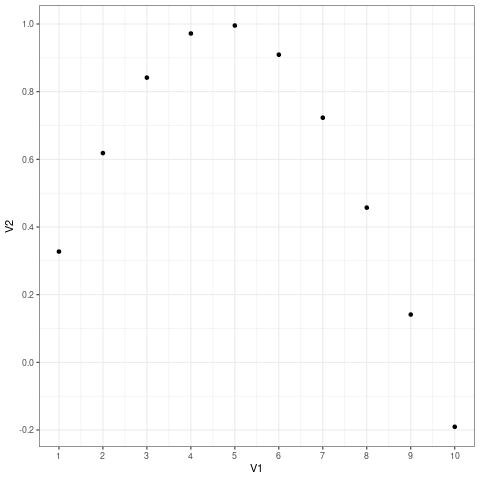
\includegraphics[width=0.8\textwidth]{figure/sin_ggplot2_breaks.png}
\end{center}

\item labelの設定
\label{sec:orge2ea547}
\begin{minted}[frame=lines,framesep=2mm,linenos=true,baselinestretch=1.2,fontsize=\footnotesize,breaklines]{r}
plt_label <- plt_breaks + xlab("x") + ylab("y")
plt_label
\end{minted}

\begin{center}
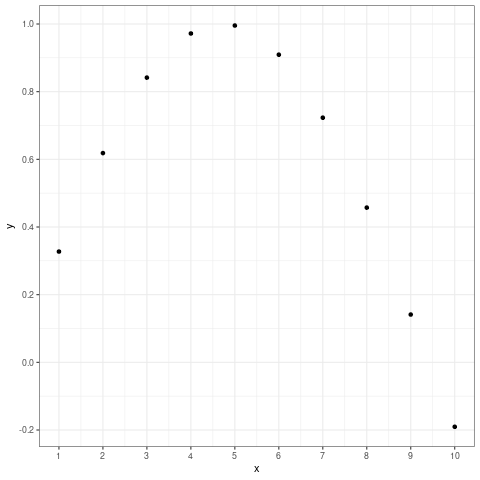
\includegraphics[width=0.8\textwidth]{figure/sin_ggplot2_label.png}
\end{center}

\item aesの中でshapeとかcolorを指定するとlegendが出る
\label{sec:org7eb2bbc}

\begin{itemize}
\item \texttt{\%+\%} で既存の要素を置き換えられるらしい.
\end{itemize}


\begin{minted}[frame=lines,framesep=2mm,linenos=true,baselinestretch=1.2,fontsize=\footnotesize,breaklines]{r}
plt_legend <- plt_label %+%
  aes(shape = "サイン", color = "サイン")
plt_legend
\end{minted}

\begin{center}
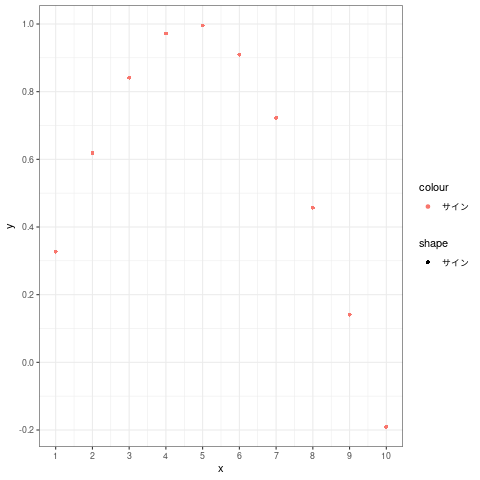
\includegraphics[width=0.8\textwidth]{figure/sin_ggplot2_legend.png}
\end{center}

\item shapeとcolorを変える
\label{sec:org2105af2}
\begin{minted}[frame=lines,framesep=2mm,linenos=true,baselinestretch=1.2,fontsize=\footnotesize,breaklines]{r}
plt_legend2 <- plt_legend +
  scale_shape_manual("functions", values = c(3)) +
  scale_color_manual("functions", values = c("#990066"))
plt_legend2
\end{minted}

\begin{center}
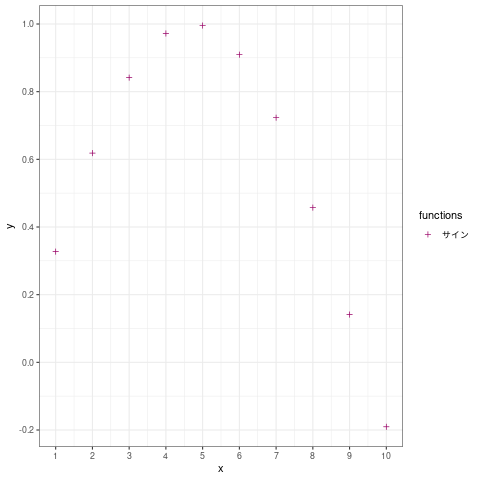
\includegraphics[width=0.8\textwidth]{figure/sin_ggplot2_legend2.png}
\end{center}

\item legendの位置を変更
\label{sec:org0cb0059}

legendの左下(0.0, 0.0)を図の(0.1, 0.1)へ持っていく.
\begin{minted}[frame=lines,framesep=2mm,linenos=true,baselinestretch=1.2,fontsize=\footnotesize,breaklines]{r}
plt_legend_position <- plt_legend2 +
  theme(legend.justification = c(0.0, 0.0)
      , legend.position      = c(0.1, 0.1))
plt_legend_position
\end{minted}

\begin{center}
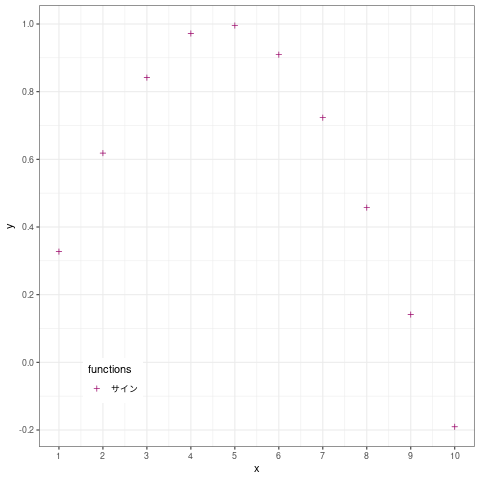
\includegraphics[width=0.8\textwidth]{figure/sin_ggplot2_legend_position.png}
\end{center}

\item legendに囲みを変更
\label{sec:orgcc82ee9}
\begin{minted}[frame=lines,framesep=2mm,linenos=true,baselinestretch=1.2,fontsize=\footnotesize,breaklines]{r}
plt_legend_box <- plt_legend_position +
  theme(legend.background     = element_blank()
      , legend.box.background = element_rect(color = "black"))
plt_legend_box
\end{minted}

\begin{center}
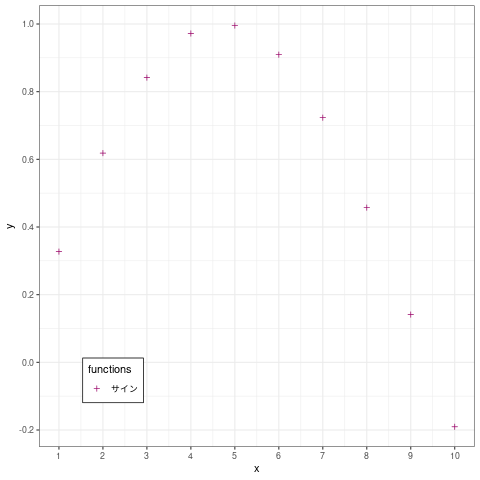
\includegraphics[width=0.8\textwidth]{figure/sin_ggplot2_legend_box.png}
\end{center}

\item 文字を大きく, 色を黒に
\label{sec:org386d13d}
\begin{minted}[frame=lines,framesep=2mm,linenos=true,baselinestretch=1.2,fontsize=\footnotesize,breaklines]{r}
plt_text_prop <- plt_legend_box +
  theme(legend.text  = element_text(size = 20)
      , legend.title = element_text(size = 20)
      , axis.text  = element_text(size = 20, color = "black")
      , axis.title = element_text(size = 24))
plt_text_prop
\end{minted}

\begin{center}
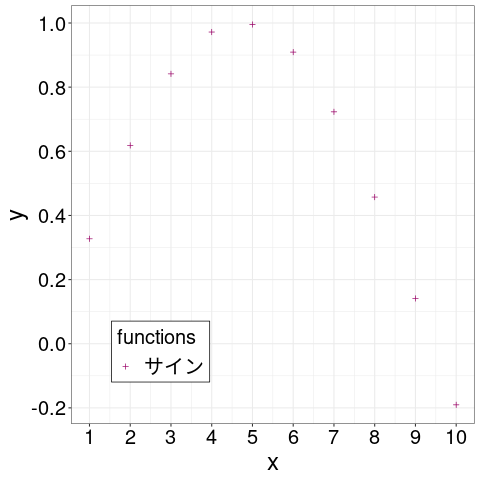
\includegraphics[width=0.8\textwidth]{figure/sin_ggplot2_text_prop.png}
\end{center}

\item legendのタイトルとグリッドを消去する
\label{sec:orge4ed6aa}
\begin{minted}[frame=lines,framesep=2mm,linenos=true,baselinestretch=1.2,fontsize=\footnotesize,breaklines]{r}
plt_grid <- plt_text_prop +
  theme(legend.title = element_blank()
      , panel.grid = element_blank())
plt_grid
\end{minted}

\begin{center}
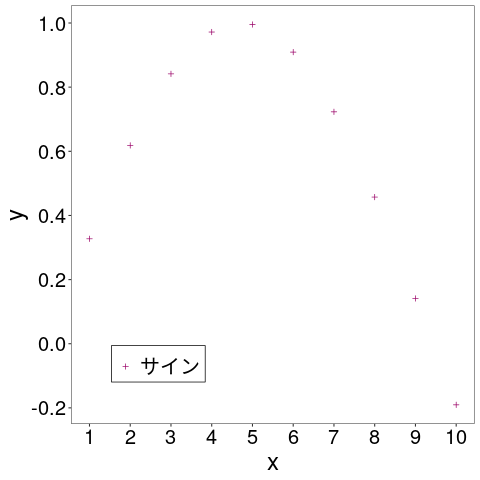
\includegraphics[width=0.8\textwidth]{figure/sin_ggplot2_grid.png}
\end{center}

\item ticksを内側に変更する.
\label{sec:org28eff1a}

ticksのテキストのマージンも変更する.
\begin{minted}[frame=lines,framesep=2mm,linenos=true,baselinestretch=1.2,fontsize=\footnotesize,breaklines]{r}
plt_ticks <- plt_grid +
  theme(axis.text.x  = element_text(margin = margin(t = 0.5, unit = "cm"))
      , axis.text.y  = element_text(margin = margin(r = 0.5, unit = "cm"))
      , axis.ticks.length=unit(-0.25, "cm"))
plt_ticks
\end{minted}

\begin{center}
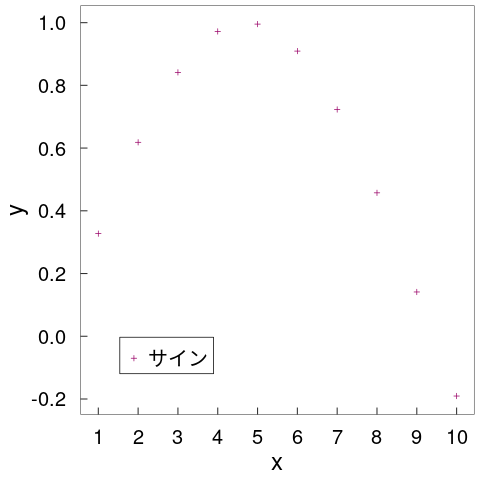
\includegraphics[width=0.8\textwidth]{figure/sin_ggplot2_ticks.png}
\end{center}

\item アスペクト比を変更する
\label{sec:org51186c7}
\begin{minted}[frame=lines,framesep=2mm,linenos=true,baselinestretch=1.2,fontsize=\footnotesize,breaklines]{r}
plt_aspect <- plt_ticks +
  theme(aspect.ratio = 3/4)
plt_aspect
\end{minted}

\begin{center}
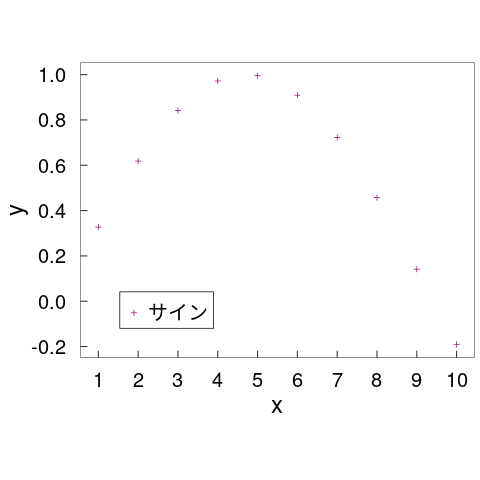
\includegraphics[width=0.8\textwidth]{figure/sin_ggplot2_aspectratio.png}
\end{center}

\item 比較
\label{sec:org8a449ff}

\begin{itemize}
\item 結構似ている.
\item ここまでする必要はないが, 色々自由に設定できる.
\end{itemize}

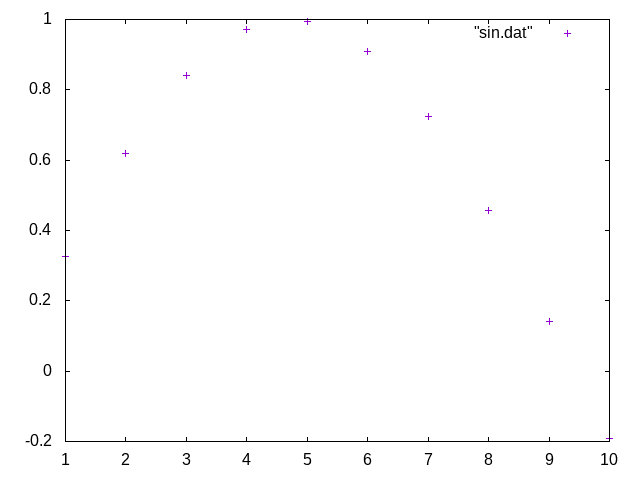
\includegraphics[width=0.45\textwidth]{figure/sin_gnuplot.png}
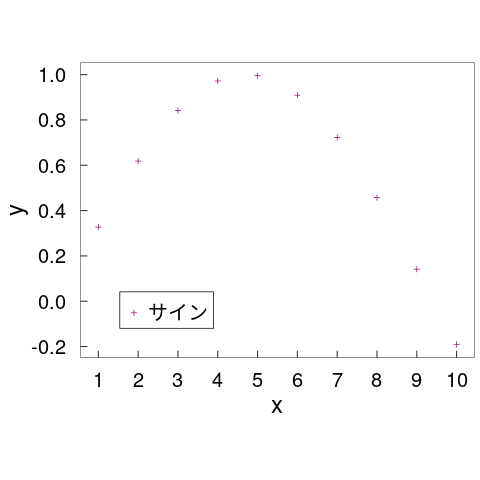
\includegraphics[width=0.45\textwidth]{figure/sin_ggplot2_aspectratio.png}
\end{enumerate}
\subsection{ファイルに書き込む}
\label{sec:org2257e73}
\subsubsection{gnuplotなら}
\label{sec:orgfcbdd5c}
\begin{minted}[frame=lines,framesep=2mm,linenos=true,baselinestretch=1.2,fontsize=\footnotesize,breaklines]{gnuplot}
set size square
set terminal png
set output 'sin_gnuplot_output.png'
plot "sin.dat" using 1:2 with points
\end{minted}

\begin{center}
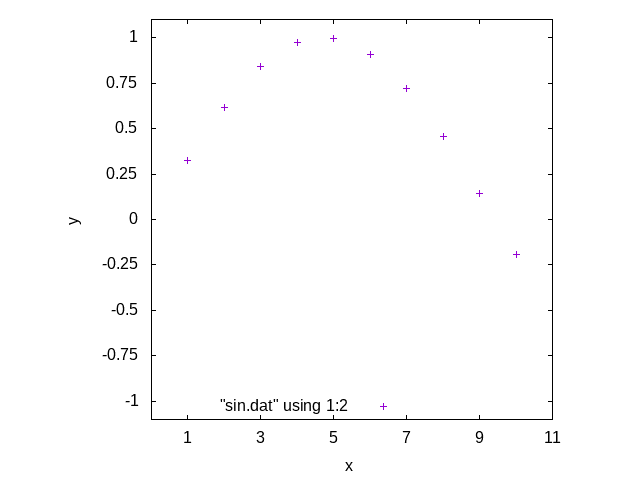
\includegraphics[width=0.8\textwidth]{sin_gnuplot_output.png}
\end{center}
\subsubsection{R+ggplot2}
\label{sec:org822e8b0}
\begin{minted}[frame=lines,framesep=2mm,linenos=true,baselinestretch=1.2,fontsize=\footnotesize,breaklines]{r}
plt <- ggplot(data = d_sin) + geom_point(aes(x = V1, y = V2))
ggsave(filename = "sin_ggplot2_output.png"
     , plot = plt
     , width = 7, height = 7)
\end{minted}

\begin{center}
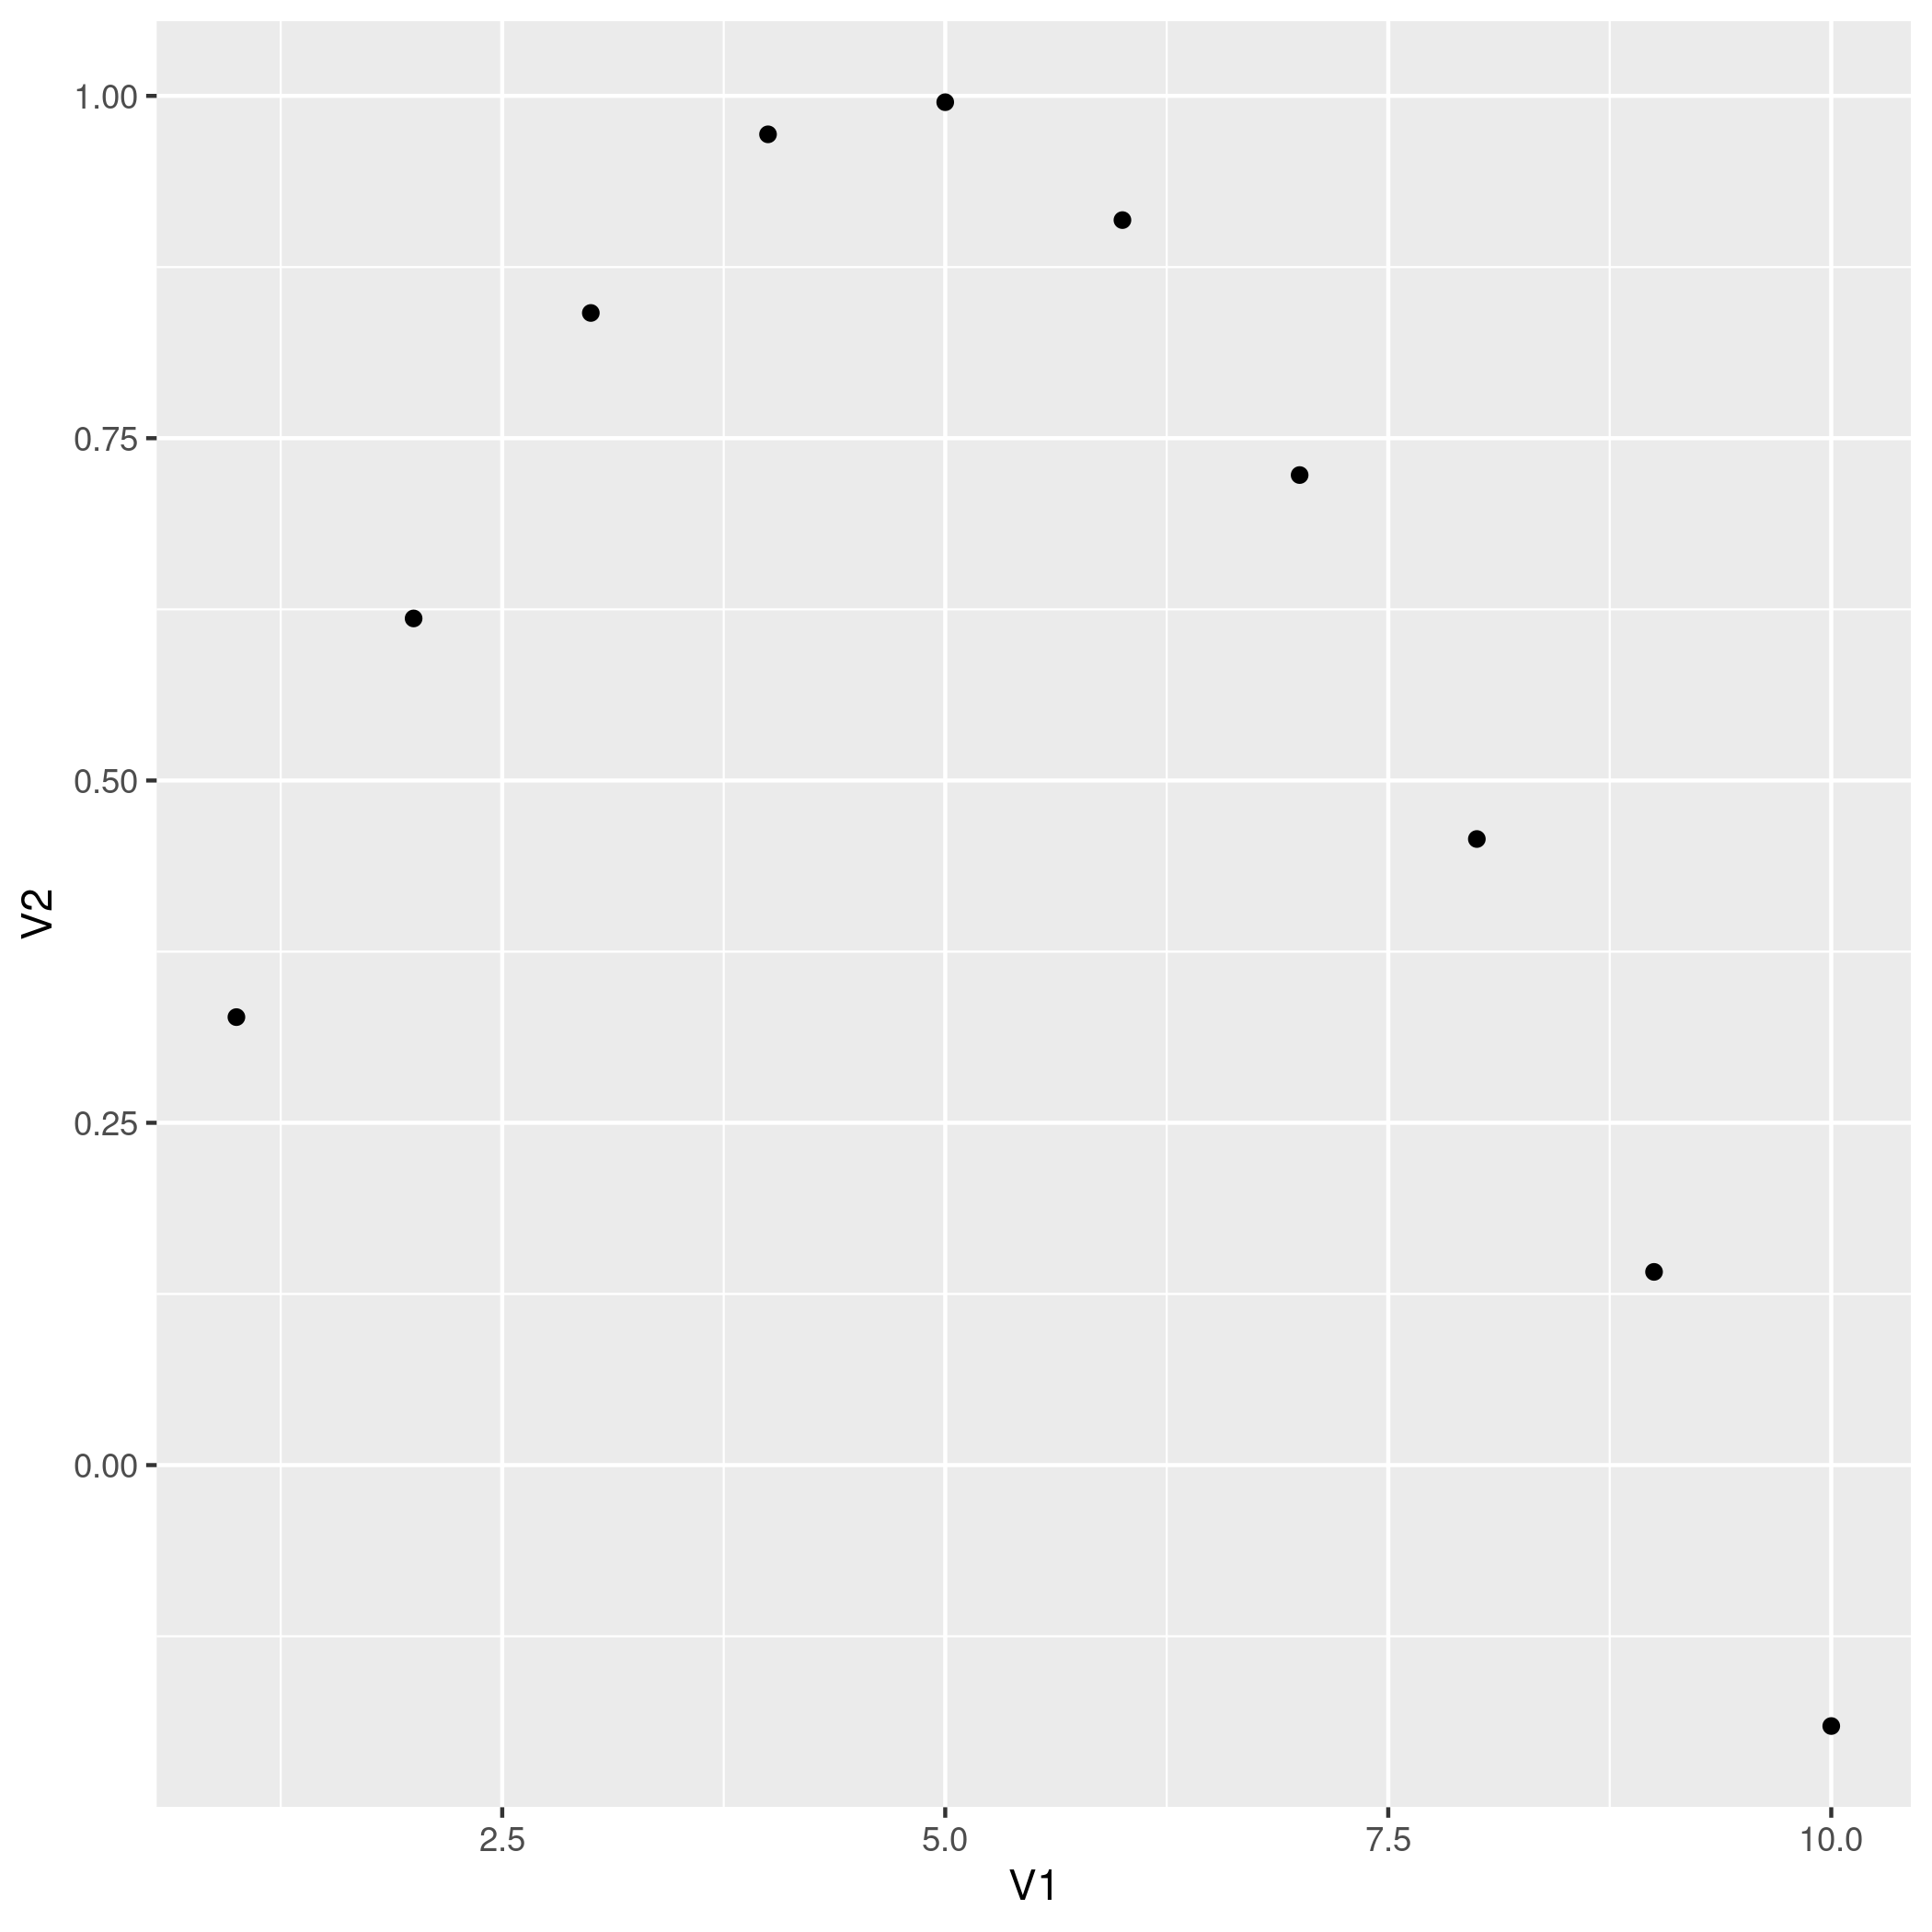
\includegraphics[width=0.8\textwidth]{sin_ggplot2_output.png}
\end{center}
\subsection{範囲を指定}
\label{sec:orgfa94efe}
\subsubsection{gnuplotなら}
\label{sec:orga07cc31}
\begin{minted}[frame=lines,framesep=2mm,linenos=true,baselinestretch=1.2,fontsize=\footnotesize,breaklines]{gnuplot}
set size square
set xrange [0:11]
set yrange [-1.1:1.1]
set xtics 2
set ytics 0.2
set xlabel "x"
set ylabel "y"
set key left bottom
plot "sin.dat" using 1:2 with linespoints title "sin"
\end{minted}

\begin{center}
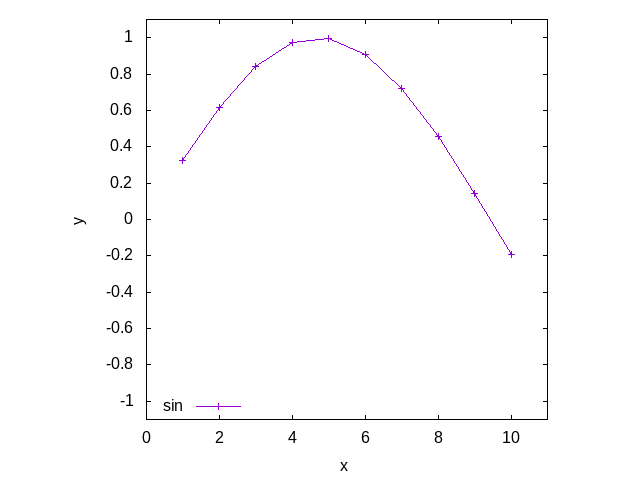
\includegraphics[width=0.8\textwidth]{figure/sin_gnuplot_range.png}
\end{center}

\subsubsection{R+ggplot2}
\label{sec:orgd8b32ea}
\begin{itemize}
\item 行末に \texttt{+} を置くと行を跨げる.
\item \texttt{geom\_point} と \texttt{geom\_line} を同時に使える.
\item \texttt{scale\_x\_continuous} と \texttt{scale\_y\_continuous} の引数 \texttt{breaks} と \texttt{limits} にベクトル \mintinline[frame=lines,framesep=2mm,linenos=true,baselinestretch=1.2,fontsize=\footnotesize,breaklines]{r}{c(...)} を渡す.

\begin{itemize}
\item \texttt{limits} に渡すのは2要素のベクトル.
\end{itemize}
\item \texttt{scale\_shape\_manual} と \texttt{scale\_color\_manual} の引数 \texttt{values} にベクトルを渡す.

\begin{itemize}
\item gnuplotのlinetypeやlinecolorみたいなもの.
\item shapeやcolorの数文の長さのベクトルが必要.
\end{itemize}
\end{itemize}
\begin{minted}[frame=lines,framesep=2mm,linenos=true,baselinestretch=1.2,fontsize=\footnotesize,breaklines]{r}
plt_range <- ggplot(data = d_sin, aes(x = V1, y = V2, shape = "sin", color = "sin")) +
  geom_point() + geom_line() +
  scale_x_continuous(breaks = seq(from = 0.0 , to = 10.0, by = 2.0)
                   , limits = c(0, 11)) +
  scale_y_continuous(breaks = seq(from = -1.0, to = 1.0 , by = 0.2)
                   , limits = c(-1.0, 1.0)) +
  scale_shape_manual("functions", values = c(3)) +
  scale_color_manual("functions", values = c("#990066")) +
  xlab("x") + ylab("y") +
  theme_bw() +
  theme(axis.text  = element_text(size = 20, color = "black")
      , axis.title = element_text(size = 20)
      , legend.text  = element_text(size = 20)
      , legend.title = element_blank()
      , legend.justification = c(0.0, 0.0)
      , legend.position      = c(0.05, 0.05)
      , panel.grid = element_blank()
      , axis.ticks.length = unit(-0.25, "cm")
      , axis.text.x       = element_text(margin = margin(t = 0.5, unit = "cm"))
      , axis.text.y       = element_text(margin = margin(r = 0.5, unit = "cm")))
plt_range
\end{minted}

\begin{center}
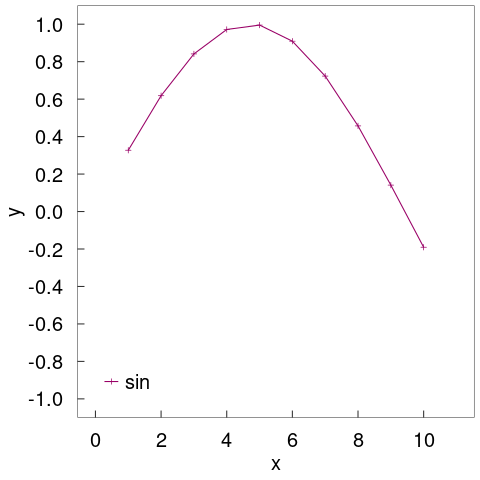
\includegraphics[width=0.8\textwidth]{figure/sin_ggplot2_range.png}
\end{center}

\subsection{複数ファイルをプロット}
\label{sec:orgd751ea8}
\subsubsection{gnuplot}
\label{sec:orgbc94c58}
\begin{minted}[frame=lines,framesep=2mm,linenos=true,baselinestretch=1.2,fontsize=\footnotesize,breaklines]{gnuplot}
set size square
set xrange [0:11]
set yrange [-1.1:1.1]
set xtics    1,    2, 11
set ytics -1.0, 0.25, 1.0
set xlabel "x"
set ylabel "y"
set key left bottom
plot "sin.dat" using 1:2 with linespoints title "sin",\
     "cos.dat" using 1:2 with linespoints title "cos"
\end{minted}

\begin{center}
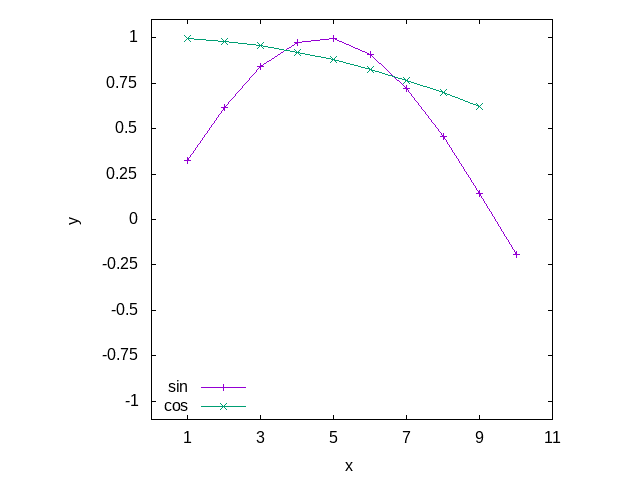
\includegraphics[width=.9\linewidth]{figure/sincos_gnuplot_multifile.png}
\end{center}

\subsubsection{R+ggplot2}
\label{sec:orgd247584}
\begin{enumerate}
\item 愚直に
\label{sec:org00a1e5a}

\begin{itemize}
\item themeを使いまわすために, \texttt{mytheme} 変数に代入しておくことができる.

xとyのscaleも使いまわす.
\end{itemize}
\begin{minted}[frame=lines,framesep=2mm,linenos=true,baselinestretch=1.2,fontsize=\footnotesize,breaklines]{r}
d_cos <- read.table("cos.dat", header = F)

mytheme <-
  theme(axis.text  = element_text(size = 20, color = "black")
      , axis.title = element_text(size = 20)
      , legend.text  = element_text(size = 20)
      , legend.title = element_blank()
      , legend.justification = c(0.0, 0.0)
      , legend.position      = c(0.05, 0.05)
      , panel.grid = element_blank()
      , axis.ticks.length = unit(-0.25, "cm")
      , axis.text.x       = element_text(margin = margin(t = 0.5, unit = "cm"))
      , axis.text.y       = element_text(margin = margin(r = 0.5, unit = "cm")))

my_x_scales <-
  scale_x_continuous(breaks = seq(from = 1.0 , to = 11.0, by = 2.0)
                   , limits = c(0, 11))
my_y_scales <-
  scale_y_continuous(breaks = seq(from = -1.0, to = 1.0 , by = 0.25)
                   , limits = c(-1.0, 1.0))

plt_multifile <- ggplot() +
  geom_point(data = d_sin, aes(x = V1, y = V2, shape = "sin", color = "sin")) +
  geom_line(data = d_sin, aes(x = V1, y = V2, shape = "sin", color = "sin")) +
  geom_point(data = d_cos, aes(x = V1, y = V2, shape = "cos", color = "cos")) +
  geom_line(data = d_cos, aes(x = V1, y = V2, shape = "cos", color = "cos")) +
  my_x_scales + my_y_scales +
  scale_shape_manual("functions", values = c(3:4)) +
  scale_color_manual("functions", values = c("#990066", "#009900")) +
  xlab("x") + ylab("y") +
  theme_bw() + mytheme
plt_multifile
\end{minted}

\begin{center}
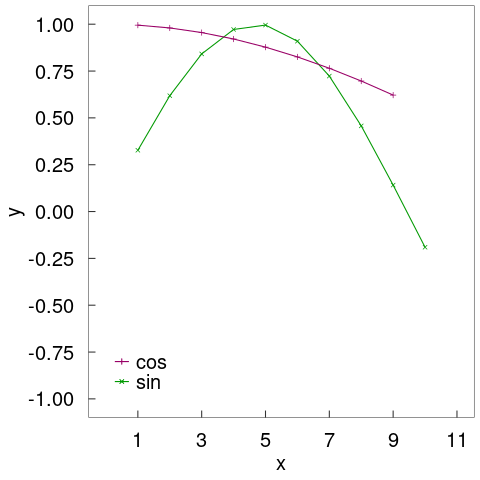
\includegraphics[width=0.8\textwidth]{figure/sincos_ggplot2_multifile.png}
\end{center}

\item data.frameの構造を変えてプロット
\label{sec:org917cef1}

\begin{itemize}
\item \texttt{data.frame} に新しい列に関数の種類を文字列で代入する.
\item \texttt{rbind} で2つを合体させる.
\end{itemize}
\begin{minted}[frame=lines,framesep=2mm,linenos=true,baselinestretch=1.2,fontsize=\footnotesize,breaklines]{r}
d_sin2 <- d_sin
d_cos2 <- d_cos
d_sin2$func <- "sin"
d_cos2$func <- "cos"
d_sincos <- rbind(d_sin2, d_cos2)
d_sincos
\end{minted}

\begin{center}
\begin{tabular}{rrl}
V1 & V2 & func\\
\hline
1 & 0.3271947 & sin\\
2 & 0.6183698 & sin\\
3 & 0.8414710 & sin\\
4 & 0.9719370 & sin\\
5 & 0.9954079 & sin\\
6 & 0.9092974 & sin\\
7 & 0.7230859 & sin\\
8 & 0.4572726 & sin\\
9 & 0.1411200 & sin\\
10 & -0.1905680 & sin\\
1 & 0.9950042 & cos\\
2 & 0.9800666 & cos\\
3 & 0.9553365 & cos\\
4 & 0.9210610 & cos\\
5 & 0.8775825 & cos\\
6 & 0.8253356 & cos\\
7 & 0.7648422 & cos\\
8 & 0.6967067 & cos\\
9 & 0.6216100 & cos\\
\hline
\end{tabular}
\end{center}

\begin{itemize}
\item \texttt{shape} と \texttt{color} に \texttt{func} を指定する.

\mintinline[frame=lines,framesep=2mm,linenos=true,baselinestretch=1.2,fontsize=\footnotesize,breaklines]{r}{"sin"} と \mintinline[frame=lines,framesep=2mm,linenos=true,baselinestretch=1.2,fontsize=\footnotesize,breaklines]{r}{"cos"} で分別する.
\end{itemize}
\begin{minted}[frame=lines,framesep=2mm,linenos=true,baselinestretch=1.2,fontsize=\footnotesize,breaklines]{r}
plt_onedataframe <- ggplot(data = d_sincos
                         , aes(x = V1, y = V2, shape = func, color = func)) +
  geom_point() + geom_line() +
  my_x_scales + my_y_scales +
  scale_shape_manual("functions", values = c(3:4)) +
  scale_color_manual("functions", values = c("#990066", "#009900")) +
  xlab("x") + ylab("y") +
  theme_bw() + mytheme
plt_onedataframe
\end{minted}

\begin{center}
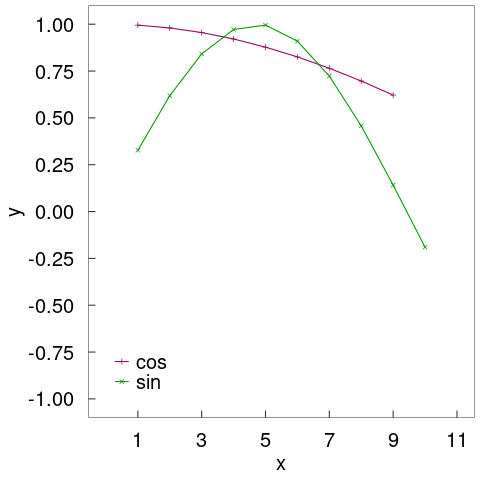
\includegraphics[width=0.8\textwidth]{figure/sincos_ggplot2_onedataframe.png}
\end{center}
\end{enumerate}

\section{まとめ}
\label{sec:orge31994b}
\begin{itemize}
\item 基本的には \mintinline[frame=lines,framesep=2mm,linenos=true,baselinestretch=1.2,fontsize=\footnotesize,breaklines]{r}{ggplot(data = mydata)} に色々足していけばよい.

\mintinline[frame=lines,framesep=2mm,linenos=true,baselinestretch=1.2,fontsize=\footnotesize,breaklines]{r}{geom_point} や \mintinline[frame=lines,framesep=2mm,linenos=true,baselinestretch=1.2,fontsize=\footnotesize,breaklines]{r}{geom_line} とか.
\item \mintinline[frame=lines,framesep=2mm,linenos=true,baselinestretch=1.2,fontsize=\footnotesize,breaklines]{r}{aes(x = myx, y = myy)} でデータフレームのどの列を使うかを指定する.

shape とか color とかも指定できる.
\end{itemize}
\section{もっと}
\label{sec:orga69d9d6}
\subsection{参考URL}
\label{sec:orgaeddc17}
\begin{itemize}
\item ggplot2のマニュアル

\url{https://cran.r-project.org/web/packages/ggplot2/ggplot2.pdf}

\item Matplotlib VS Ggplot2

matplotlib と ggplot2 との比較.

\url{https://towardsdatascience.com/matplotlib-vs-ggplot2-c86dd35a9378}
\end{itemize}
\subsection{プロットをマウスとかで弄るには}
\label{sec:org6077224}
gnuplotではプロットをマウスでぐりぐりできるが, ggplot2ではplotlyみたいなライブラリが必要.

\url{https://plotly.com/r/}

ggplotguiみたいなライブラリを使えばブラウザ上でグリグリしたり, プロットの設定を弄ったりできる.

\url{https://cran.r-project.org/web/packages/ggplotgui/README.html}

他にも色々あるらしい.

\url{https://note.com/tqwst408/n/n82d56c69a18e}
\subsection{プロットを横とか縦に並べるには}
\label{sec:orgc9eb46d}
patchworkライブラリを使うとよい.

\url{https://cran.r-project.org/web/packages/patchwork/patchwork.pdf}

\url{https://qiita.com/nozma/items/4512623bea296ccb74ba}
\end{document}